% ============================================================
%  §4  Core Equations
% ============================================================

\section{Core Equations}
\label{sec:core}

\subsection{Field Evolution}

The time evolution of the information density field is governed by:
\begin{equation}
  \frac{\partial I}{\partial\tau} + \nabla\cdot\JI = \sigma,
  \label{eq:I_evolution}
\end{equation}
where the information flow is
\begin{equation}
  \JI = -D\nabla I + \mu F_I, \qquad F_I = -\nabla\Phi = \alpha\nabla C,
  \label{eq:JI}
\end{equation}
and the generation term decomposes as
\begin{equation}
  \sigma = \sigma_{\mathrm{drive}} - \sigma_{\mathrm{dissip}} - \sigma_{\mathrm{barrier}}.
  \label{eq:sigma}
\end{equation}

The three contributions are:
\begin{align}
  \sigma_{\mathrm{drive}}  &= a\Delta\!\left(1 - \frac{C}{C_*}\right),
  \label{eq:sigma_drive}\\
  \sigma_{\mathrm{dissip}} &= \Gamma C,
  \label{eq:sigma_dissip}\\
  \sigma_{\mathrm{barrier}}&= \frac{\kappa_B}{\Cmax - C}.
  \label{eq:sigma_barrier}
\end{align}

Here $C_*$ denotes the effective saturation scale of conceptual
quasi-closure within the observation window, while $\Cmax$ denotes the
ideal complete-closure boundary.
In general $C_* < \Cmax$ for conceptual regimes.

In the cognitive domain:
$\sigma_{\mathrm{drive}}$ represents the influx of novel input
(perception, linguistic perturbation, reward signal);
$\sigma_{\mathrm{dissip}}$ represents the natural decay of
unresolved tension (forgetting, habituation);
$\sigma_{\mathrm{barrier}}$ represents a projected or coarse-grained
effective resistance against conceptual overclosure.
It should not be read as a fundamental external prohibition; it is the
cognitive-domain analogue of the effective barrier notation used in
VED and IFGT.

\subsection{Token--Field Coupling}

A purely continuous information field cannot sustain stable, low-cost
recursion: re-entering a prior field configuration is generically
expensive and drift-prone.
Stable recursion requires discrete, re-addressable structures that allow
the system to re-invoke complex field states at low cost.
Figure~\ref{fig:token-field-coupling} illustrates this local coupling
mechanism.

\begin{figure}[t]
  \centering
  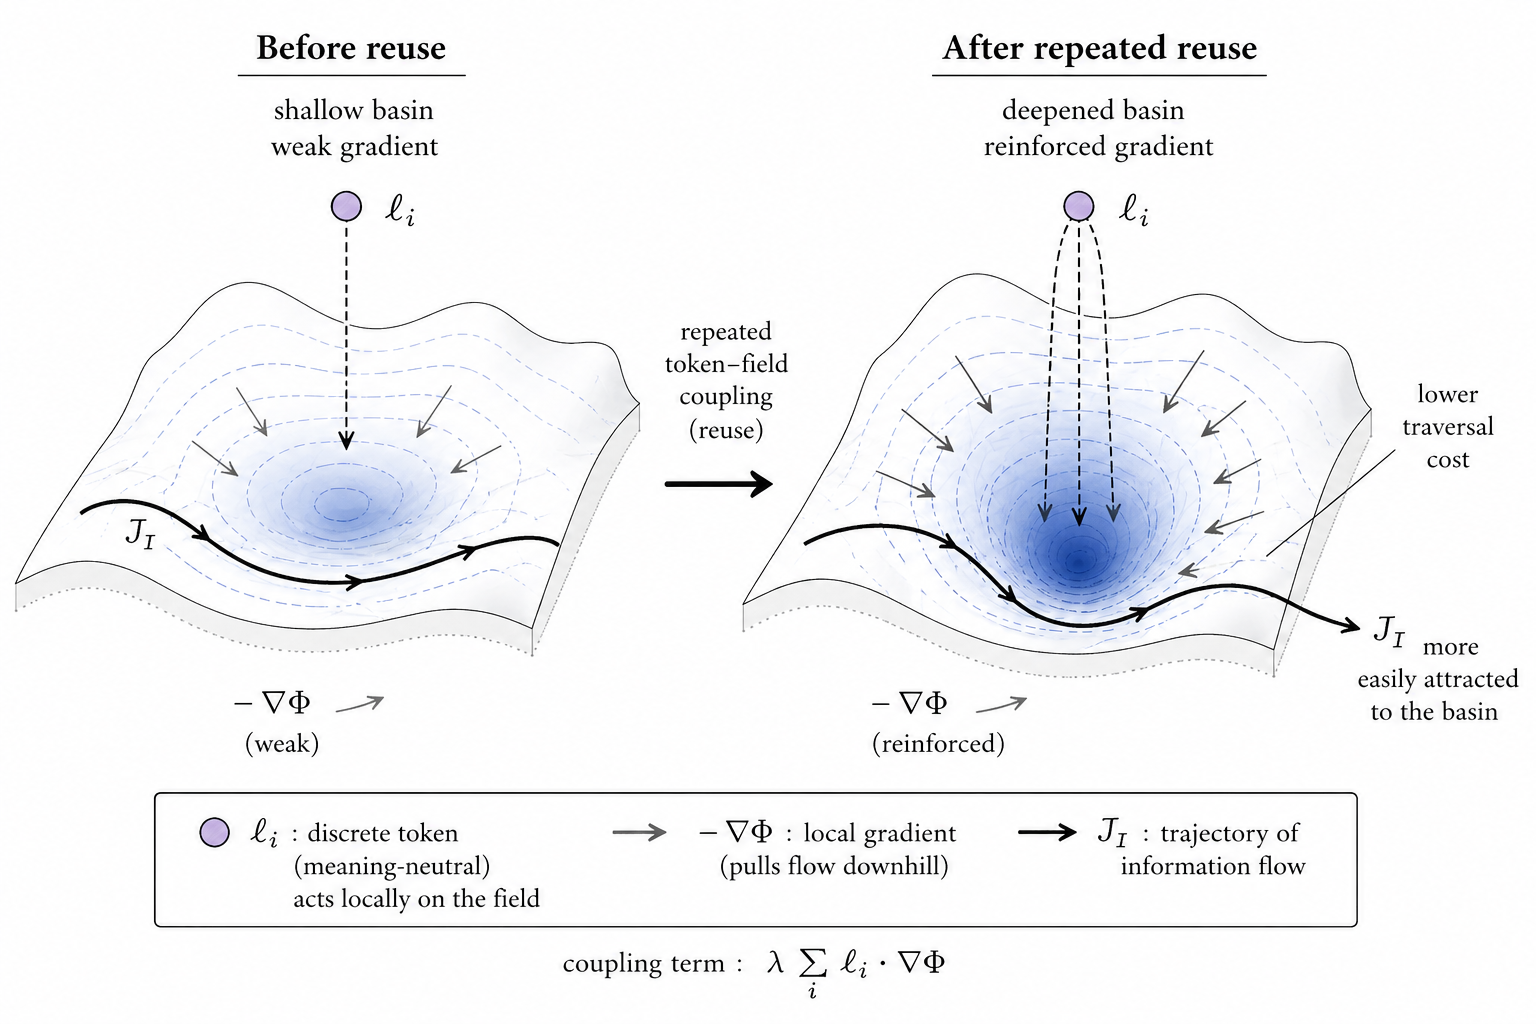
\includegraphics[width=0.95\linewidth]{figures/fig2_token_field_coupling.png}
  \caption{
  Token--field coupling and basin deepening.
  Discrete linguistic tokens $\ell_i$ do not carry semantic content; they act as re-addressable units that couple locally to $\nabla\Phi$.
  Repeated reuse reinforces local gradients, deepens the associated potential basin, and lowers traversal cost for future trajectories of $J_I$.
  The coupling is summarized by the effective term $\lambda \sum_i \ell_i \cdot \nabla\Phi$.
  }
  \label{fig:token-field-coupling}
\end{figure}

The medium that enables this structure is the linguistic field, where
``linguistic'' is understood broadly to include not only natural language
but any discrete, re-addressable medium capable of acting on the field
as a localized perturbation: symbols, emblems, gestures, diagrams,
mathematical notation, and so on.

Linguistic tokens $\ell_i$ (discrete units drawn from any such medium)
couple to the field through the gradient of the potential:
\begin{equation}
  \mathcal{L}_{\mathrm{eff}} = \mathcal{L}_{\mathrm{field}}[I]
  + \mathcal{L}_{\mathrm{token}}[\ell]
  + \lambda \sum_i \ell_i \cdot \nabla\Phi.
  \label{eq:coupling}
\end{equation}

This coupling is purely dynamical: tokens do not encode meanings but
bias the local evolution of $\Phi$ through repeated interaction.
Each token reuse reinforces the local gradient, deepening the
associated potential well.

\subsection{Sedimentation and Conceptual Landscape Formation}

Under repeated token--field interaction, the potential field
approaches a long-time attractor:
Figure~\ref{fig:minimal-recursive-loop} summarizes the irreversible loop
assumed throughout this paper.

\begin{figure}[t]
  \centering
  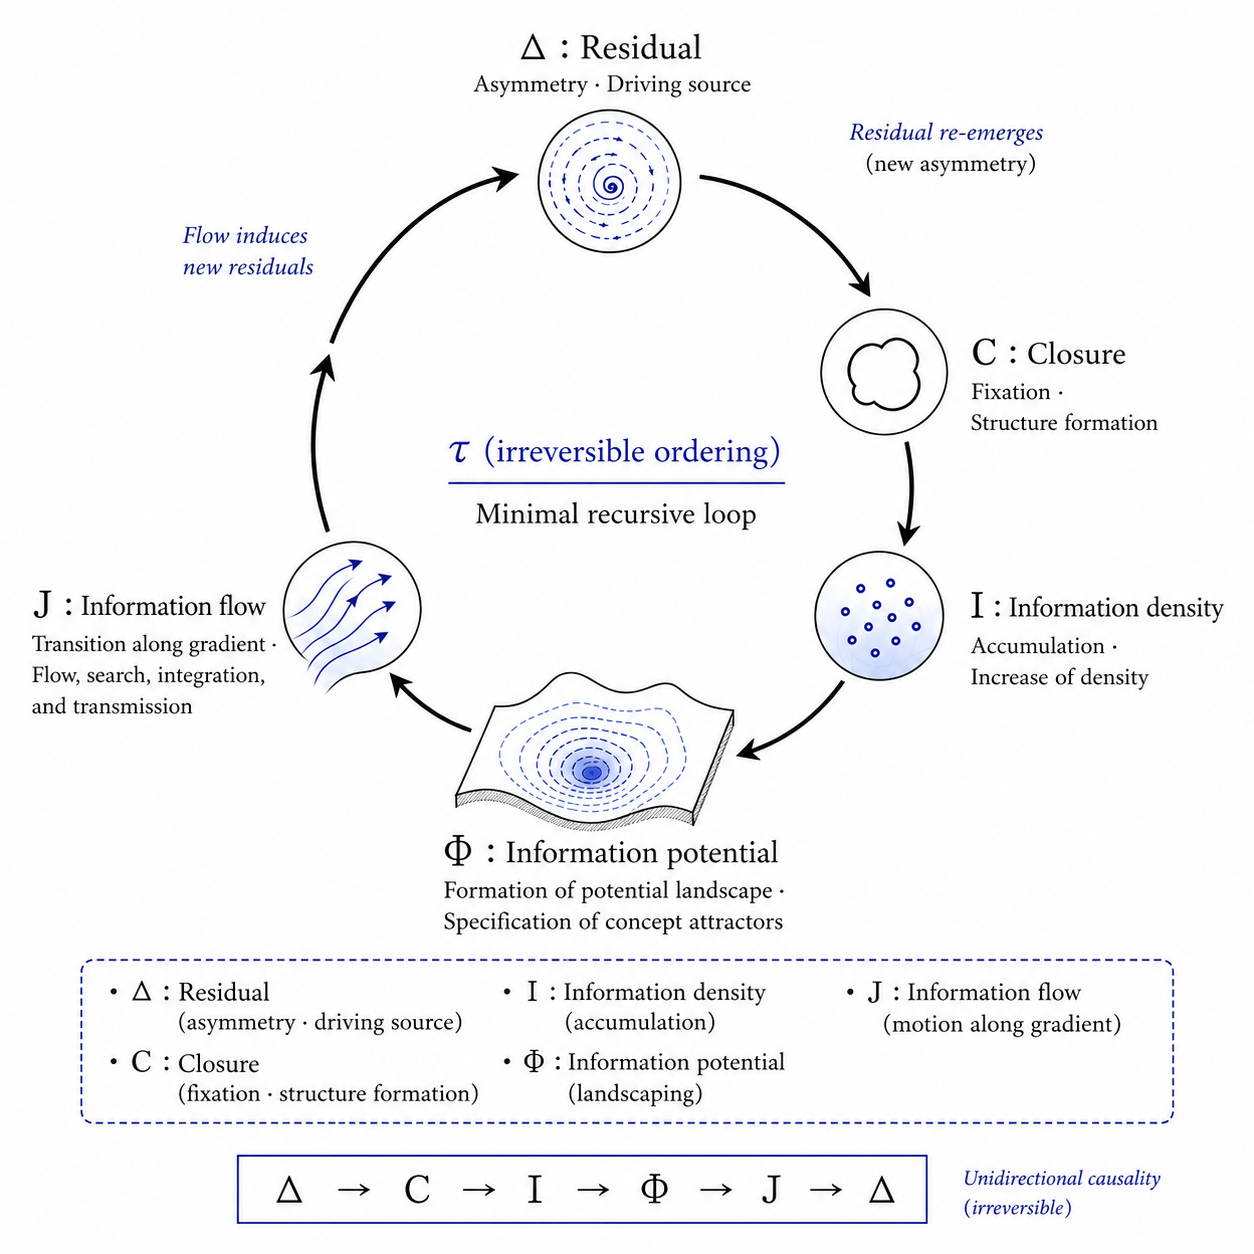
\includegraphics[width=0.82\linewidth]{figures/fig3_minimal_recursive_loop.png}
  \caption{
  Minimal recursive loop of the VED$\times$IFGT framework.
  The system evolves through the irreversible cycle
  $\Delta \to C \to I \to \Phi \to J_I \to \Delta$,
  where residual asymmetry $\Delta$ drives closure $C$, leading to information density $I$, formation of potential structure $\Phi$, and subsequent information flow $J_I$, which regenerates residuals.
  The loop is unidirectional and governed by irreversible ordering $\tau$.
  }
  \label{fig:minimal-recursive-loop}
\end{figure}

\begin{equation}
  \Phi(x,\tau) \;\xrightarrow{\;\tau\to\infty\;}\; \Phistar(x).
  \label{eq:sedimentation}
\end{equation}

$\Phistar$ is the sedimented conceptual landscape.
It is not necessarily unique or static; it reflects the history of
all prior interactions and continues to be reshaped by new input,
though at decreasing rate as the landscape matures.

\subsection{Concept Definition}

\begin{definition}[Concept]
A \emph{concept} at position $x$ is a locally stable region of the
information potential satisfying:
\begin{equation}
  \nabla\Phi(x) \approx 0, \qquad
  \text{with stability under small perturbations of } \JI.
  \label{eq:concept}
\end{equation}
The depth of the potential well at $x$ measures the concept's
resistance to deformation; its width measures its contextual range.
\end{definition}

\begin{definition}[Understanding]
\emph{Understanding} a conceptual region $\mathcal{R}$ is the state
in which the traversal cost of $\JI$ through $\mathcal{R}$ has been
reduced to below a system-dependent threshold $\theta$:
\begin{equation}
  \int_{\mathcal{R}} |\nabla\Phi|\,dx < \theta.
  \label{eq:understanding}
\end{equation}
Here $\theta$ is a system-dependent effective threshold expressing the
allowable range of recursive cost.
Its concrete value depends on the structure of the system, including
$D$, $\mu$, $\alpha$, and related parameters, and is not specified in
the present work.
Understanding is not a binary state but a dynamical condition that can
be entered and exited as $\Phi$ evolves.
\end{definition}

\subsection{The Strict Positivity Constraint}

The structural positivity of the information field,
\begin{equation}
  \boxed{I(x,\tau) > 0 \qquad \forall\,x,\,\tau,}
  \label{eq:positivity}
\end{equation}
follows from $C < \Cmax$ combined with $I = f(1-C) > 0$ for
$C < \Cmax$.
Here $\Cmax$ denotes the ideal complete-closure boundary, not an
ordinary attainable state of the conceptual system.

\begin{proposition}[No ordinary complete conceptual closure]
Under the VED$\times$IFGT framework, $I>0$ excludes complete conceptual
closure as an ordinary dynamical state.
In nontrivial generated landscapes with residual asymmetry,
spatial inhomogeneity, or boundary structure, this residual positivity
generically appears as nonzero gradients in $\Phi$ and hence as
available directions for $\JI$.
The proposition should therefore be read as a statement about the
non-attainability of final conceptual stasis, not as the pointwise
mathematical claim that every positive $I$ must have
$\nabla\Phi\neq0$.
\end{proposition}

\begin{remark}
This result has direct implications for theories of intelligence and
understanding: no conceptual landscape is finished in the sense of
reaching complete closure.
Stable attractors may appear locally quiescent, but they remain embedded
in a generated field where further differentiation can reappear under
new perturbations or wider observation windows.
\end{remark}
